%----------------------------------------------------------------------------
%----------------------------------------------------------------------------
It has become clear that the main issue one must deal with to prepare a commercial dye laser for use in a multi-color coherent control experiment is the multi-mode nature of these sources. The processes under investigation demand transform limited pulses \cite{Corless:1997a} and well controlled intensity profiles. The raw output of each of the three dye lasers is unusable since it is not transform limited, has non--Gaussian anti-symmetric transverse intensity profiles ($M^2$ not close to unity), and cannot be arbitrarily delayed with respect to the pump laser. To condition each beam for use in the experiment, we temporally condition the pulse into a Gaussian shape, run the pulse through a variable delay line, spatially filter the beam to eliminate the non-TEM00 transverse modes ($M^2 \sim 1$), then spectrally filter the pulse to its transform limit (see figure \ref{block_dye}).
%----------------------------------------------------------------------------
% block_dye.tex.tex
% by Troy Hix, May 2005
%----------------------------------------------------------------------------
\begin{figure}
\center
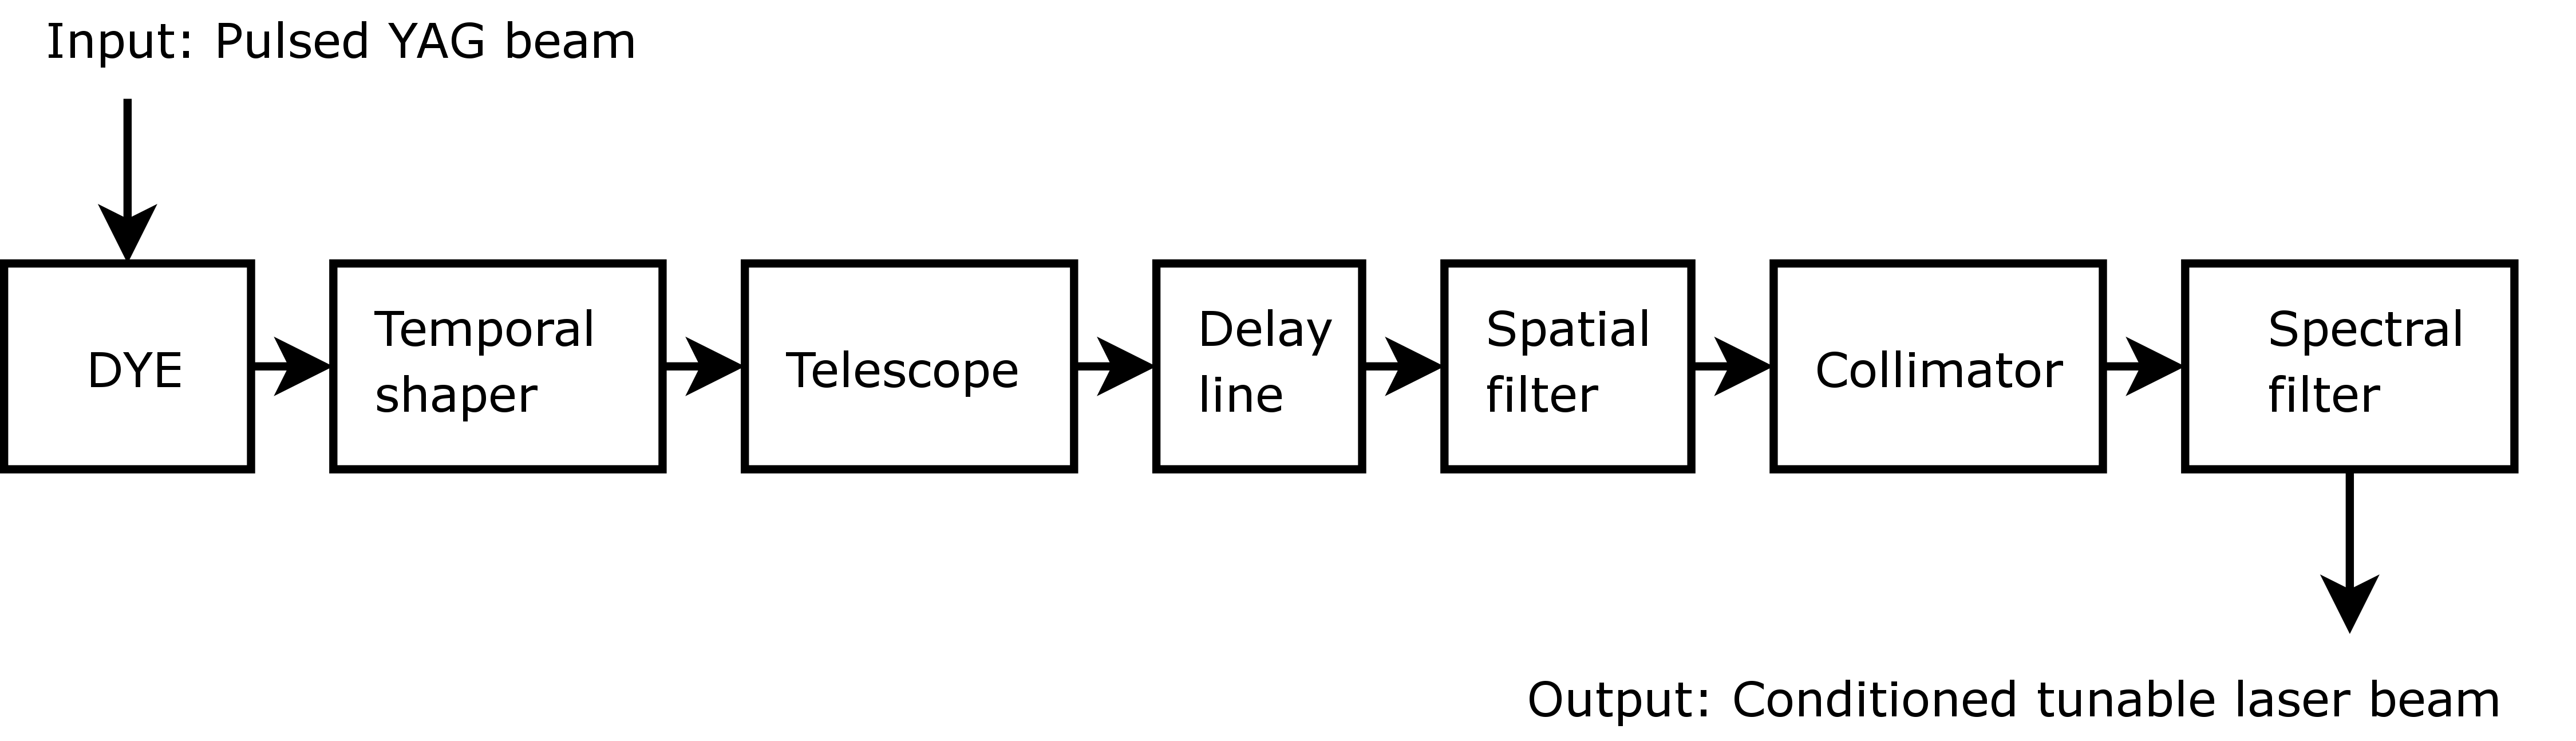
\includegraphics[width=6.00in]
{block_dye/block_dye.png}\\
\caption{Single dye laser conditioning block diagram}
\label{block_dye}
\end{figure} 
%----------------------------------------------------------------------------
%----------------------------------------------------------------------------
%----------------------------------------------------------------------------



%----------------------------------------------------------------------------

The temporal shaper is a Pockels cell (the Pockels cell will also be used to set the amplitude of each pulse). It has been shown in the lab that the Pockels cell can create dye laser pulses with widths from 0.8 ns to 4.4 ns. The lower limit is a characteristic of the Pockels cell and its associated electronics; the upper limit is roughly the longest pulse we are able to generate when we eliminate the ragged leading and trailing edges of the raw laser output. For transform limited shapes (Gaussians), the temporal FWHM of the intensity is related to the spectral FWHM of the power spectrum by
%----------------------------------------------------------------------------
\begin{equation}
\boxed{
\sigma_\nu
=
\frac
{\ln(16)}
{2\pi\sigma_t},
\label{FWHM power}
}
\end{equation}
%----------------------------------------------------------------------------
where $\sigma_\nu$ is the spectral FWHM and $\sigma_t$ is the temporal FWHM.

Thus, if $\sigma_t$ is 0.8 ns then $\sigma_\nu$ is 552 MHz, and if $\sigma_t$ is 4.4 ns then $\sigma_\nu$ is 100 MHz. These are the target spectral filter widths for long and short pulse experiments. The spectral filters are etalons with a FSR big enough to prevent aliasing and a mode width of 100 MHz to 552 MHz depending on the type of experiment.

The delay line extends the path length of the beam in such a manner to allow arbitrary delay between the dye laser pulse and YAG pump. A telescope is used upstream from the delay line to minimize the effect of the variable path length between the dye laser output and the spatial filter. The spatial filter is placed downstream from the delay line and shall consist of a focusing lens and a pinhole. The central maximum from the pinhole (Airy function) is mode matched into the etalon (beam is collimated if a planar configuration is used - or focused if confocal). Then the beam is finally collimated (if necessary) and sent to the molecular interaction region.
%----------------------------------------------------------------------------
%----------------------------------------------------------------------------
%----------------------------------------------------------------------------
%----------------------------------------------------------------------------
%----------------------------------------------------------------------------
%----------------------------------------------------------------------------
